\documentclass[11pt]{article}

% --- encoding / fonts -------------------------------------------------------
\usepackage[utf8]{inputenc}
\usepackage[T1]{fontenc}
\usepackage{lmodern}
\usepackage[margin=1in]{geometry}

% --- math / graphics / tables ----------------------------------------------
\usepackage{amsmath,amssymb,mathtools}
\usepackage{graphicx}
\graphicspath{{figures/}}
\usepackage{booktabs}
\usepackage{algorithm}
\usepackage{algpseudocode}
\usepackage{xcolor}
\usepackage{caption}

% --- hyperlinks / cross-references (load hyperref before cleveref) ----------
\usepackage[colorlinks=true,linkcolor=blue!45!black,citecolor=blue!45!black,%
            urlcolor=blue!45!black]{hyperref}
\usepackage{cleveref}

% --- schematic --------------------------------------------------------------
\usepackage{tikz}
\usetikzlibrary{arrows.meta,calc}

% --- convenience macros (keep notation identical to the code) ---------------
\newcommand{\vth}{v_{\mathrm{thresh}}}
\newcommand{\vr}{v_{\mathrm{rest}}}
\newcommand{\vre}{v_{\mathrm{reset}}}
\newcommand{\vmin}{v_{\min}}
\newcommand{\teff}{\theta_{\mathrm{eff}}}
\newcommand{\thetaevent}{\theta_{\mathrm{event}}}
\newcommand{\rinf}{r_{\infty}}
\newcommand{\Gb}{G_{b}}
\newcommand{\Gbase}{G_{\mathrm{base}}}
\newcommand{\Gdyn}{G_{\mathrm{dyn}}}
\newcommand{\Jdb}{J_{\mathrm{DB}}}
\newcommand{\code}[1]{\texttt{#1}}

\title{\textbf{A Mathematically Consistent, Nengo-Compatible Reference\\
Implementation of HyperLIF and Adaptive HyperLIF Neurons:\\
Exact Validation, Capability Coverage, and\\
Operating-Point Calibration}}

\author{%
  Adaptive HyperLIF / Nengo Research Project\\
  \small Companion implementation and validation study to the Adaptive HyperLIF theory manuscript~\cite{hyperlif_theory}
}
\date{\today}

\begin{document}
\maketitle

\begin{abstract}
The leaky integrate-and-fire (LIF) neuron resets its membrane potential
discontinuously at threshold, which is convenient for simulation but makes the
state evolution non-smooth and obscures the sub-threshold ``readiness'' state of the
neuron. The companion theory manuscript~\cite{hyperlif_theory} replaces the
hard reset with a continuous, gate-controlled discharge, yielding the
\emph{HyperLIF} neuron and its input-stabilized variant, \emph{Adaptive
HyperLIF}. This paper contributes a clean, self-contained, and rigorously
validated reference implementation of those neurons that is compatible with the
Neural Engineering Framework toolkit Nengo~\cite{bekolay2014nengo}. We restate
the implemented equations exactly as coded, expose two numerical stepping
schemes---an explicit-Euler scheme matching the Julia reference and an
exponential-Euler scheme used by the Nengo port---and analyze their accuracy and
stability against a fine Runge--Kutta reference. A frozen-open-gate equilibrium
analysis gives the branch estimate
$\Jdb=(\vth-\gamma)(1+\tau\Gb)=2.4$ for the reference parameters and the branch
voltage $v^\ast=J/(1+\tau\Gb)$; the voltage prediction matches the simulated
high-drive latch (e.g.\ $v^\ast=1.3333$ predicted and observed at $J=4$). The
adaptive conductance law bounds the positive-drive, $r=1$ asymptotic branch below
the gate knee when $\beta>1/(\tau(\vth-\gamma))=62.5$ (here $\beta=80$). This
changes the high-drive regime but is not a global-stability or firing theorem.
We further show that the standalone exponential stepping
and the Nengo custom-neuron stepping agree to floating-point exactness (voltage
and gate RMSE $=0$, zero event-timing mismatch) across two stimulus protocols
and both models, because both call an identical numerical kernel. We then evaluate the neurons across the breadth of Nengo. In canonical
integrator/oscillator smoke tests the base HyperLIF holds only weakly---but we
show this is an \emph{operating-point} artifact: with readout calibration (a
separate event threshold $\thetaevent=0.95$, an origin offset, and a fitted
rate-to-current gain), HyperLIF integrates and holds, and \emph{exceeds} LIF on
an amplitude-matched oscillator and a gated working memory, at roughly
$3.5\times$ fewer spikes. All nine canonical capability classes---representation,
dynamics, memory, online learning, and cognition (binding and action
selection)---run with HyperLIF as a drop-in \code{NeuronType}; its one weakness
is online-learning speed, which we show is a tunable firing-rate trade with a
$\sim\!40$ Hz sweet spot. A five-seed scalar NEF state-readout ablation then
shows that the probeable reset gate and combined state features can decode the
represented signal at low firing rates. A static $\thetaevent=0.95$ raises the
peak settled event rate from $151.14$ to $217.83$ Hz without changing the
continuous gate/reset dynamics. We further find a hard framework limit: a custom
continuous-gate neuron is confined to the reference NumPy simulator---the OpenCL
and Loihi backends reject it and NengoDL is version-locked---so accelerated or
neuromorphic deployment would require per-backend kernels or a fixed-hardware
neuron mapping. Finally, we interpret the continuous reset gate as a decodable
readiness-to-fire signal, an explicitly future-work bridge to gate-state residual
decoding for control. All figures, tables, and claims are reproducible from the
included code and data.
\end{abstract}

% ===========================================================================
\section{Introduction}\label{sec:intro}
% ===========================================================================
The discontinuous threshold-and-reset rule of the LIF
neuron~\cite{lapicque1907} makes spike generation a hybrid (non-smooth)
dynamical process. This is the root cause of two practical difficulties. First,
the reset map is not differentiable, so gradient-based training of spiking
networks must either approximate the missing derivative with surrogate
gradients~\cite{neftci2019surrogate} or handle spike events explicitly with
specialized adjoint machinery~\cite{wunderlich2021eventprop}. Second, the
instantaneous jump discards information: the moment the membrane reaches
threshold, its trajectory is overwritten, leaving only the emitted event as an
observable. The continuous-reset \emph{HyperLIF} family introduced in the
companion theory manuscript~\cite{hyperlif_theory} removes the discontinuity by
modeling the reset as a fast but smooth, gate-controlled discharge, producing a
continuous-state ordinary differential equation (ODE) system with an explicit,
interpretable internal gate state $r(t)$. The binary event observable remains
non-differentiable; event-dependent losses require a surrogate or an explicit
event-time derivative. Adaptive HyperLIF also contains a non-smooth $|J|$ term
at $J=0$ unless it is regularized.

Theory and benchmark performance for the HyperLIF family are reported in
\cite{hyperlif_theory}. The present paper addresses a complementary and equally
important question for downstream use: \emph{can these continuous-reset neurons
be implemented as a clean, equation-faithful, and numerically validated
component of a standard neural-engineering workflow?} We answer this
affirmatively by building a small reference package that (i) implements LIF,
HyperLIF, and Adaptive HyperLIF from a single mathematical specification, (ii)
ports HyperLIF and Adaptive HyperLIF to Nengo~\cite{bekolay2014nengo} as custom
\code{NeuronType} classes with probeable continuous state, and (iii) validates
the port against the standalone implementation to floating-point exactness. The
Neural Engineering Framework (NEF)~\cite{eliasmith2003neural} that underlies
Nengo provides a principled route from encoded stimuli to decoded estimates, and
has been used for closed-loop adaptive robot control~\cite{dewolf2016reach}; a
validated HyperLIF \code{NeuronType} is the prerequisite for using the
continuous gate state inside that workflow.

\paragraph{Contributions.} This paper makes the following contributions.
\begin{enumerate}
  \item A single-source, equation-faithful reference implementation of LIF,
  HyperLIF, and Adaptive HyperLIF, with every manuscript equation traceable to
  specific lines of code (\Cref{sec:formulation,sec:lif,sec:hyperlif,sec:adaptive}).
  \item A closed-form characterization of the frozen open-gate equilibrium:
  the branch estimate $\Jdb=(\vth-\gamma)(1+\tau\Gb)$ and branch voltage
  $v^\ast=J/(1+\tau\Gb)$, checked against high-drive simulation, and the
  condition $\beta>1/(\tau(\vth-\gamma))$ under which the adaptive positive-drive,
  $r=1$ asymptote lies below the gate knee
  (\Cref{sec:hyperlif,sec:adaptive,sec:results-fi}).
  \item An analysis of the two discrete stepping schemes (explicit-Euler vs.\
  exponential-Euler) against a Runge--Kutta reference, quantifying convergence
  and contractivity of its frozen scalar exponential substep
  (\Cref{sec:integration,sec:results-integration}).
  \item A demonstration that the Nengo port reproduces the standalone
  exponential stepping \emph{exactly} (voltage/gate RMSE $=0$, zero event
  mismatch) across protocols and models, with an explanation grounded in a
  shared numerical kernel (\Cref{sec:nengo,sec:results-parity}).
  \item A first NEF application smoke test showing that LIF, HyperLIF, and
  Adaptive HyperLIF build and run inside canonical Nengo integrator/oscillator
  models; the apparent weak base-HyperLIF integrator response is shown in
  \Cref{sec:capability} to be an operating-point artifact, not a dynamics limit
  (\Cref{sec:results-nef,sec:thetaevent}).
  \item A capability-coverage and operating-point-calibration study
  (\Cref{sec:capability}): with a calibrated readout ($\thetaevent$, origin, and
  a fitted rate-to-current gain), HyperLIF runs all nine canonical Nengo
  capability classes---representation, dynamics, memory, online learning, and
  cognition (binding, action selection)---matching or \emph{exceeding} LIF on
  dynamics and memory at $\sim\!3.5\times$ fewer spikes, with online-learning
  speed identified as a tunable firing-rate trade.
  \item A five-seed scalar NEF state-readout ablation
  (\Cref{tab:nef-decoder-ablation}): the calibrated HyperLIF reset gate and
  combined state readouts carry decodable represented-signal information at much
  lower firing rates than native LIF.
  \item A backend-portability characterization
  (\Cref{sec:capability-backend}): a custom continuous-gate \code{NeuronType}
  runs only in the reference NumPy simulator; the OpenCL and Loihi backends
  reject it and NengoDL is version-locked, delimiting where the component can
  currently be deployed.
  \item An interpretation of the reset gate as a decodable readiness-to-fire
  signal, and an explicitly-labeled future-work bridge to gate-state residual
  decoding for control (\Cref{sec:readiness,sec:bridge}).
\end{enumerate}

% ===========================================================================
\section{Motivation and Background}\label{sec:background}
% ===========================================================================
\subsection{From hard reset to continuous reset}
A standard LIF neuron integrates its input and, upon crossing $\vth$, is reset
to $\vre$ instantaneously. The companion theory~\cite{hyperlif_theory} reframes
this jump as the standard-real projection of an infinitesimal-time discharge,
producing a stiff two-time-scale ODE in which a fast gate variable $r(t)$
mediates a continuous reset conductance. Enforcing continuity exposes dynamical
regimes that the idealized hybrid abstraction hides---most notably a
depolarization block (DB), a silent depolarized mode under sustained strong
drive that is well documented in biophysical
models~\cite{bianchi2012db,dovzhenok2012db} and is the continuous-system
resolution of a Zeno-like accumulation of reset events~\cite{zhang2001zeno}. The
Adaptive HyperLIF changes the high-drive branch over the intended operating range by
scaling the reset conductance with input magnitude. We take these models as
given and focus on a faithful, validated realization.

\subsection{Why Nengo compatibility matters}
Nengo~\cite{bekolay2014nengo} implements the NEF~\cite{eliasmith2003neural}:
populations of neurons encode signals through tuning curves and decode them
through learned linear weights. Implementing HyperLIF as a Nengo
\code{NeuronType} places the continuous-reset neuron inside this standard
ecosystem---probeable state, calibrated gains/biases, and ensemble decoding---so
that the gate state can be used as a decodable feature alongside spikes and
voltage. Because NEF-based spiking controllers have been demonstrated for
adaptive robotic control~\cite{dewolf2016reach}, a validated port is the natural
substrate for the attitude-control direction discussed in \Cref{sec:bridge}.

\subsection{Notation}
\Cref{tab:notation} fixes the notation, which is identical to the symbols used
in the code and in \cite{hyperlif_theory}. Unless stated otherwise we use the
normalized convention $\vr=\vre=0$, $\vth=1$, so $J$ and the conductance $G$ are
dimensionless relative to the leak term.
\begin{table}[t]
\centering
\caption{Notation used throughout the paper.}
\label{tab:notation}
\begin{tabular}{l p{0.72\columnwidth}}
\toprule
Symbol & Meaning \\
\midrule
$v(t)$ & Membrane voltage (normalized) \\
$r(t)\in[0,1]$ & Continuous reset gate (fast activation-like proxy) \\
$J$ (= $I_{\mathrm{in}}$) & Net input current / drive (normalized) \\
$\tau,\ \tau_r$ & Membrane and gate time constants ($\tau_r\ll\tau$) \\
$v_{\mathrm{rest}},v_{\mathrm{reset}},v_{\mathrm{thresh}}$ & Rest, reset, threshold voltages \\
$\sigma(\cdot)$ & Logistic gate detector, steepness $\alpha$ \\
$\gamma,\ \theta_{\mathrm{eff}}$ & Hysteresis and effective threshold $\theta_{\mathrm{eff}}=v_{\mathrm{thresh}}-\gamma r$ \\
$G_b$ & Fixed reset gain (baseline HyperLIF) \\
$G_{\mathrm{base}},\ \beta$ & Baseline gain and adaptive scaling (Adaptive HyperLIF) \\
$G(r,J)$ & Reset conductance scale; $G_b r^2$ or $(G_{\mathrm{base}}+\beta|J|)r^2$ \\
$G_{\mathrm{dyn}}$ & Adaptive conductance scale $G_{\mathrm{base}}+\beta|J|$ \\
$\lambda$ & Membrane relaxation rate $1/\tau + G$ \\
$J_{\mathrm{DB}}$ & Frozen-open-gate DB branch estimate \\
$\Delta t$ & Simulation time step \\
\bottomrule
\end{tabular}
\end{table}


% ===========================================================================
\section{Mathematical Formulation}\label{sec:formulation}
% ===========================================================================
All three neuron models share the membrane/leak structure; they differ in how
the reset is realized. We state each model exactly as implemented. A compact
qualitative comparison is given in \Cref{tab:modelcompare}, and the default
parameters (reflected directly from the parameter dataclasses) in
\Cref{tab:params}.
\begin{table*}[t]
\centering
\caption{Qualitative comparison of the three neuron models in the reference implementation.}
\label{tab:modelcompare}
\small
\begin{tabular}{p{0.17\textwidth} p{0.23\textwidth} p{0.24\textwidth} p{0.25\textwidth}}
\toprule
Property & LIF & HyperLIF & Adaptive HyperLIF \\
\midrule
State variables & $\{v\}$ & $\{v, r\}$ & $\{v, r\}$ \\
Reset mechanism & hard jump to $v_{\mathrm{reset}}$ & gate conductance $G_b r^2$ & input-modulated $(G_{\mathrm{base}}+\beta|J|)r^2$ \\
Threshold event & discontinuous & smooth crossing & smooth crossing \\
Continuous \& differentiable & no (hybrid) & yes & yes \\
Refractory handling & explicit $\tau_{\mathrm{ref}}$ & gate hysteresis $\gamma$ & gate hysteresis $\gamma$ \\
High-drive behaviour & increasing firing & high-voltage latch & bounded subthreshold dynamics \\
Nengo \texttt{NeuronType} & (built-in) & \texttt{HyperLIFNengo} & \texttt{AdaptiveHyperLIFNengo} \\
\bottomrule
\end{tabular}
\end{table*}


% ---------------------------------------------------------------------------
\subsection{LIF baseline}\label{sec:lif}
The baseline LIF membrane obeys
\begin{equation}
  \frac{dv}{dt} = \frac{-(v-\vr) + J}{\tau}. \label{eq:lif-ode}
\end{equation}
For a sub-threshold step the implementation advances the membrane with the exact
linear update
\begin{equation}
  v_{k+1} = (\vr + J) + \big(v_k - \vr - J\big)\,e^{-\Delta t/\tau},
  \label{eq:lif-update}
\end{equation}
which is the closed-form solution of \cref{eq:lif-ode} for constant $J$. If the
membrane crosses threshold from below, $v_k<\vth\le v_{k+1}$, the neuron emits an
event of magnitude $A/\Delta t$ (Nengo's spike convention), is reset to $\vre$,
and enters a refractory interval $\tau_{\mathrm{ref}}$ during which the voltage
is held at $\vre$. The voltage is clamped from below at $\vmin$. This is a
deliberately minimal hard-reset reference for figures and decoding comparisons,
not a replacement for Nengo's production LIF.

% ---------------------------------------------------------------------------
\subsection{HyperLIF model}\label{sec:hyperlif}
HyperLIF augments the membrane with a continuous reset gate $r(t)\in[0,1]$. The
gate detector is a steep logistic with effective threshold
$\teff=\vth-\gamma r$ (a hysteresis that lowers the threshold as the gate opens):
\begin{align}
  \teff &= \vth - \gamma r, \label{eq:theta}\\
  \rinf &= \sigma\!\big(\alpha (v-\teff)\big), \quad
  \sigma(x) = \frac{1}{1+e^{-x}}. \label{eq:sigmoid}
\end{align}
The two-state continuous-time dynamics are
\begin{align}
  \frac{dr}{dt} &= \frac{\rinf - r}{\tau_r}, \label{eq:gate-ode}\\
  \frac{dv}{dt} &= \frac{-(v-\vr)+J}{\tau} - G(r)\,(v-\vre), \qquad
  G(r) = \Gb\, r^2. \label{eq:hyperlif-ode}
\end{align}
The reset conductance $G(r)=\Gb r^2$ is quadratic in the gate so that
$\partial G/\partial r = 0$ at gate onset, preserving a sharp, LIF-like upstroke
until the gate commits~\cite{hyperlif_theory}. Crucially, \emph{there is no hard
reset}: \cref{eq:hyperlif-ode} pulls the membrane toward $\vre$ continuously
through $G(r)$. Events are emitted for readout only, on an upward crossing of an
event level $v_{\mathrm{event}}$ (by default $\vth$), and do not alter the state.

\paragraph{Open-gate equilibrium and the depolarization block.}
Setting $dv/dt=0$ in \cref{eq:hyperlif-ode} for a frozen gate value $r$ and
constant $J$ gives the membrane equilibrium
\begin{equation}
  v^\ast(r) = \frac{\vr + J + \tau\,G\,\vre}{1 + \tau\,G}, \qquad G=\Gb r^2,
  \label{eq:vstar}
\end{equation}
i.e.\ the drive divided by the total (leak plus reset) conductance. Under strong
sustained drive the gate saturates open ($r\to 1$). In the normalized convention
$v^\ast(1)=J/(1+\tau\Gb)$. Equating this \emph{frozen open-gate branch}
with the gate knee $\teff(1)=\vth-\gamma$ gives the useful branch estimate
$v^\ast(1)\ge \vth-\gamma$. Solving for the corresponding current,
\begin{equation}
  \boxed{\;\Jdb = (\vth-\gamma)\,(1+\tau\Gb) - \vr - \tau\Gb\,\vre.\;}
  \label{eq:jdb}
\end{equation}
For the reference parameters ($\vth=1,\gamma=0.2,\tau=0.02,\Gb=100$),
\cref{eq:jdb} gives $\Jdb=0.8\times 3 = 2.4$, and the latched voltage at, e.g.,
$J=4$ is $v^\ast(1)=4/3=1.3333$. \Cref{sec:results-fi} confirms both numbers
against simulation.

% ---------------------------------------------------------------------------
\subsection{Adaptive HyperLIF model}\label{sec:adaptive}
Adaptive HyperLIF keeps \cref{eq:theta,eq:sigmoid,eq:gate-ode} unchanged and
replaces the fixed reset gain by an input-dependent conductance scale,
\begin{equation}
  \Gdyn = \Gbase + \beta\,|J|, \qquad
  G(r,J) = \Gdyn\, r^2 = (\Gbase + \beta\,|J|)\, r^2,
  \label{eq:adaptive-gain}
\end{equation}
so that the membrane equation becomes
\begin{equation}
  \frac{dv}{dt} = \frac{-(v-\vr)+J}{\tau} - (\Gbase + \beta\,|J|)\,r^2\,(v-\vre).
  \label{eq:adaptive-ode}
\end{equation}
The feedforward term $\beta|J|$ raises the available discharge capacity in
proportion to the drive. Substituting $G=\Gbase+\beta|J|$ with $r=1$ into
\cref{eq:vstar} and taking $|J|\to\infty$ gives the asymptotic open-gate voltage
\begin{equation}
  v^\ast_\infty = \frac{1+\tau\beta\,\vre}{\tau\beta}
  \;\xrightarrow{\;\vre=0\;}\; \frac{1}{\tau\beta}. \label{eq:vinf}
\end{equation}
If this branch limit stays below the gate knee, a fully open gate is not
self-consistent on the same high-voltage latch branch as the fixed-gain model.
The corresponding normalized branch condition is
\begin{equation}
  \boxed{\;\beta > \frac{1}{\tau\,(\vth-\gamma)}.\;} \label{eq:beta-crit}
\end{equation}
For the reference parameters the critical value is
$1/(0.02\times 0.8)=62.5$; the configured $\beta=80$ satisfies
\cref{eq:beta-crit}, and indeed $v^\ast_\infty=1/(0.02\times 80)=0.625<0.8$.
\Cref{eq:beta-crit} bounds the positive-drive, $r=1$ asymptotic equilibrium
branch. It does not by itself prove global stability, existence of a limit
cycle, or successful discharge for arbitrary time-varying or recurrent input;
those properties require analysis of the full coupled system.

% ===========================================================================
\section{Numerical Integration}\label{sec:integration}
% ===========================================================================
The gate dynamics \cref{eq:gate-ode} are stiff ($\tau_r\ll\tau$), so naive
explicit integration of the gate is inaccurate at practical step sizes. The
implementation therefore advances the gate with the \emph{exact} first-order
relaxation obtained by freezing the target $\rinf$ over one step,
\begin{equation}
  r_{k+1} = \operatorname{clip}\!\Big(\rinf + (r_k-\rinf)\,e^{-\Delta t/\tau_r},
  \; 0,\; 1\Big), \label{eq:gate-update}
\end{equation}
and then advances the membrane with one of two schemes that share this gate
update. The \textbf{exponential (``stable'') scheme} solves the membrane
equation exactly over one step, treating $J$ and the post-update conductance
$G$ as constant. Writing the membrane equation as
$\dot v = d - \lambda v$ with
\begin{equation}
  \lambda = \tfrac{1}{\tau} + G, \qquad
  d = \tfrac{\vr}{\tau} + \tfrac{J}{\tau} + G\,\vre,
  \label{eq:lambda-drive}
\end{equation}
its exact update is
\begin{equation}
  v_{k+1} = v_k\,e^{-\lambda\Delta t}
            + \frac{d}{\lambda}\,\big(1-e^{-\lambda\Delta t}\big).
  \label{eq:stable-update}
\end{equation}
The \textbf{explicit-Euler (``Julia'') scheme} instead advances the membrane
with a forward-Euler step,
\begin{equation}
  v_{k+1} = v_k + \Delta t\!\left[\frac{-(v_k-\vr)+J}{\tau} - G\,(v_k-\vre)\right].
  \label{eq:euler-update}
\end{equation}
For frozen $J$ and $G$, \cref{eq:stable-update} is the exact contractive scalar
substep (the factor $e^{-\lambda\Delta t}\in(0,1]$ for all $\Delta t>0$),
whereas \cref{eq:euler-update} is stable only for $\lambda\Delta t<2$. This
does not establish A-stability or global stability of the nonlinear coupled
operator-split map. Both schemes converge to the same continuous trajectory as
$\Delta t\to 0$ under the usual consistency and regularity conditions.
\Cref{alg:step} summarizes the per-step update; it is exactly the code path used
by both the standalone simulator (\code{method="stable"}) and the Nengo port.

\begin{algorithm}[t]
\caption{HyperLIF / Adaptive HyperLIF discrete update (one step).}
\label{alg:step}
\begin{algorithmic}[1]
\Require state $(v,r)$, input $J$, step $\Delta t$, parameters
\State $\teff \gets \vth - \gamma\,r$ \Comment{hysteresis}
\State $\rinf \gets \sigma(\alpha(v-\teff))$ \Comment{detector}
\State $r \gets \operatorname{clip}\!\big(\rinf + (r-\rinf)e^{-\Delta t/\tau_r},0,1\big)$
\State $G \gets \Gb r^2$ \; \textbf{or} \; $(\Gbase+\beta|J|)r^2$ \Comment{HyperLIF / Adaptive}
\State $\lambda \gets 1/\tau + G$;\quad $d \gets \vr/\tau + J/\tau + G\,\vre$
\State $v_{\mathrm{prev}} \gets v$
\State $v \gets v\,e^{-\lambda\Delta t} + (d/\lambda)(1-e^{-\lambda\Delta t})$
  \Comment{exponential; Euler variant: \cref{eq:euler-update}}
\State $v \gets \max(v, \vmin)$
\State $\mathrm{spike} \gets \big[\,v_{\mathrm{prev}} < v_{\mathrm{event}} \le v\,\big]$
  \Comment{readout only; no reset}
\State \Return $(v,r),\ \mathrm{spike}$
\end{algorithmic}
\end{algorithm}

% ===========================================================================
\section{Nengo Implementation}\label{sec:nengo}
% ===========================================================================
Nengo $4.1$ realizes a custom neuron through \code{NeuronType.state}: the builder
allocates one signal per declared state variable and calls
\code{step(dt, J, output, **state)} at every simulation tick. The ports declare
explicit state dictionaries---\{\code{voltage}, \code{reset\_gate},
\code{previous\_voltage}\} for \code{HyperLIFNengo}, plus \code{dynamic\_gain}
for \code{AdaptiveHyperLIFNengo}---all of which are probeable. The body of
\code{step} performs precisely lines 1--9 of \Cref{alg:step}: it computes the
effective threshold, the logistic target, the exact gate relaxation
\cref{eq:gate-update}, the conductance, and the exponential membrane update
\cref{eq:stable-update} through the same \code{stable\_voltage\_update} routine
that the standalone simulator calls. Consequently the Nengo neuron is not a
re-derivation but a re-use of one numerical kernel, which is why the agreement
reported in \Cref{sec:results-parity} is exact rather than merely close.

For ensemble use, the ports also implement NEF gain/bias calibration: the
threshold current is $\vth-\vr$, and \code{rate\_to\_current} maps a requested
maximum firing rate to a top input current, so that standard
\code{max\_rates}/\code{intercepts} specifications produce the expected tuning
curves. This calibration is not exercised by the single-neuron validation in
this paper (which injects current directly) but is required for the ensemble
decoding envisioned in \Cref{sec:bridge}.

% ===========================================================================
\section{Validation Experiments}\label{sec:experiments}
% ===========================================================================
All experiments use a single neuron driven by a prescribed current at
$\Delta t=10^{-4}\,$s unless noted, with the default parameters of
\Cref{tab:params}. The standalone simulators use \code{method="julia"} for the
dynamics figures (matching the reference stepping) and \code{method="stable"}
for the Nengo parity check. The protocols are: a single \emph{step}
($J=1.4$ on $[0.03,0.20]\,$s); a piecewise-constant \emph{stress} current
ramping to $J=4$; a constant-current \emph{sweep} over $J\in[0,6]$ at spacing
$0.1$ with the firing rate measured over a settled window $[0.15,0.6]\,$s; a
sustained \emph{DB-drive} at $J=3.3$; a smooth multi-frequency
\emph{decoding} current; and a numerical-\emph{integration} study at
$J=1.5$ against a Runge--Kutta reference at $\Delta t_{\mathrm{ref}}=2\times
10^{-6}\,$s. Each experiment writes a CSV and a log; every figure and table in
\Cref{sec:results} is generated from those CSVs and is traceable to a named
file (see the accompanying \code{FIGURE\_TABLE\_MAP.md}).

\begin{figure}[t]
  \centering
  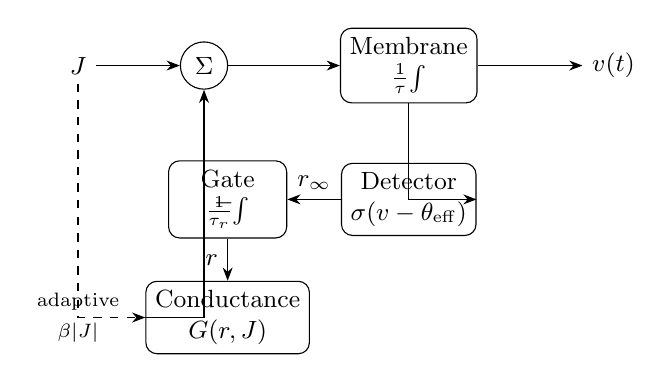
\begin{tikzpicture}[
      >=Stealth, font=\small,
      block/.style={draw, rounded corners, minimum width=15mm, minimum height=8mm, align=center},
      sum/.style={draw, circle, minimum size=6mm, inner sep=0pt}]
    % forward path
    \node (in) at (0,0) {$J$};
    \node[sum] (sum) at (1.6,0) {$\Sigma$};
    \node[block] (mem) at (4.2,0) {Membrane\\ $\tfrac{1}{\tau}\!\int$};
    \node (out) at (6.8,0) {$v(t)$};
    \draw[->] (in) -- (sum);
    \draw[->] (sum) -- (mem);
    \draw[->] (mem) -- (out);
    % feedback / reset subsystem
    \node[block] (det) at (4.2,-1.7) {Detector\\ $\sigma(v-\teff)$};
    \node[block] (gate) at (1.9,-1.7) {Gate\\ $\tfrac{1}{\tau_r}\!\int$};
    \node[block] (cond) at (1.9,-3.2) {Conductance\\ $G(r,J)$};
    \draw[->] ($(mem.south)$) |- (det.east);
    \draw[->] (det) -- (gate) node[midway,above]{$\rinf$};
    \draw[->] (gate) -- node[left]{$r$} (cond);
    \draw[->] (cond) -| (sum) node[pos=0.75,right]{$-$};
    % adaptive feedforward path
    \draw[->, dashed] (in) |- ($(cond.west)+(-0.0,0)$);
    \node[align=center] at (0.0,-3.2) {\scriptsize adaptive\\ \scriptsize $\beta|J|$};
  \end{tikzpicture}
  \caption{Signal flow of the (Adaptive) HyperLIF neuron as implemented. The
  forward path integrates the membrane; the feedback loop
  (detector $\to$ gate $\to$ conductance) implements the continuous reset through
  $r(t)$. The dashed feedforward path is the adaptive term $\beta|J|$ that scales
  the reset conductance with input magnitude (\cref{eq:adaptive-gain}); removing
  it recovers the fixed-gain HyperLIF.}
  \label{fig:schematic}
\end{figure}

% ===========================================================================
\section{Results}\label{sec:results}
% ===========================================================================

\subsection{Continuous vs.\ hard reset}\label{sec:results-step}
\Cref{fig:step} contrasts LIF and HyperLIF under the same current step. The LIF
membrane produces the familiar saw-tooth of hard resets, whereas the HyperLIF
membrane rises smoothly, hovers near threshold, and is discharged continuously
by the gate. A revealing detail is that the gate completes several
readiness cycles while only a single upward threshold crossing is registered:
the continuous reset keeps the trajectory near, but mostly below, the event
level, so the event channel under-reports the activity that the gate state makes
explicit. This already motivates treating $r(t)$ as an observable in its own
right (\Cref{sec:readiness}).

\begin{figure}[t]
  \centering
  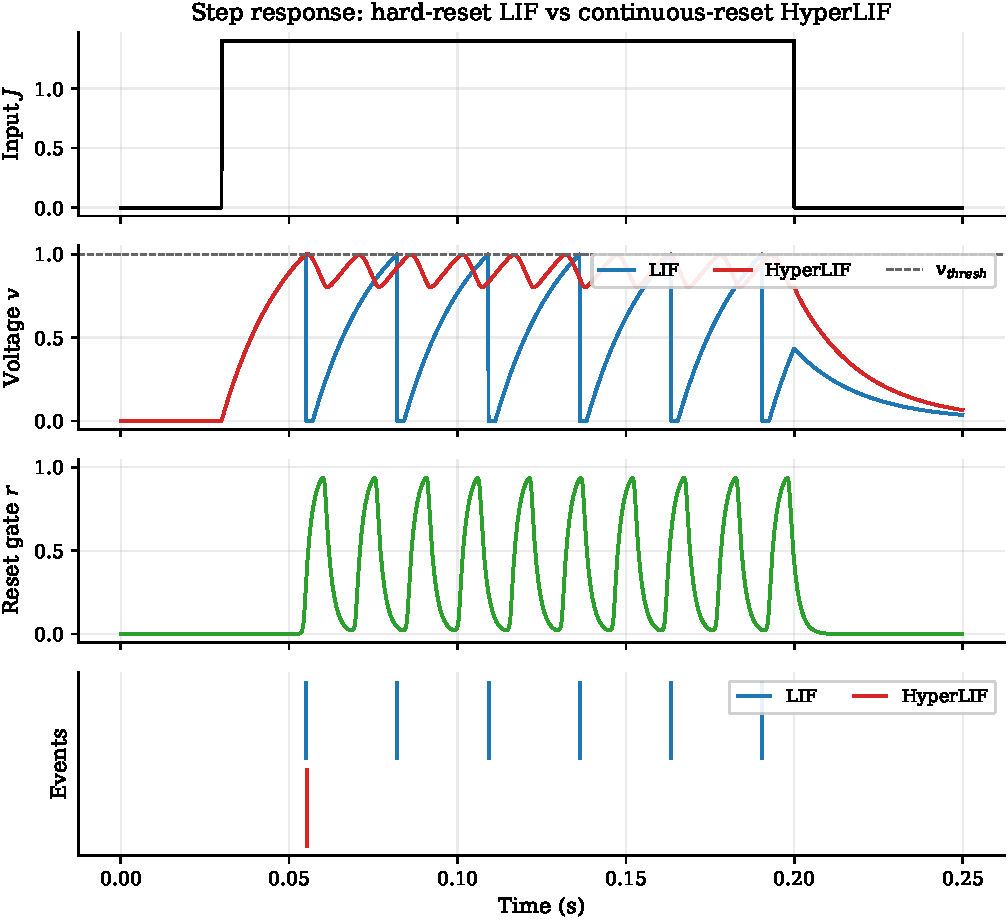
\includegraphics[width=\linewidth]{fig_step}
  \caption{Step response. Hard-reset LIF (blue) vs.\ continuous-reset HyperLIF
  (red): input current, membrane voltage with threshold, the HyperLIF reset gate
  $r(t)$, and event rasters. The gate cycles several times while only one
  HyperLIF event is registered. Source: \code{01\_lif\_vs\_hyperlif.csv}.}
  \label{fig:step}
\end{figure}

\subsection{Fixed vs.\ adaptive reset conductance}\label{sec:results-stress}
\Cref{fig:stress} drives both continuous-reset models with a stress current that
ramps to $J=4$. During the high-current phase the fixed-gain HyperLIF membrane
latches above threshold (its gate saturates and its conductance plateaus at
$\Gb=100$), i.e.\ it enters the DB. Adaptive HyperLIF instead raises its
conductance with $|J|$ (the dynamic gain $\Gdyn$ tracks the staircase input) and
keeps oscillating below threshold. This is the time-domain signature of the
operating-range expansion characterized statically next.

\begin{figure}[t]
  \centering
  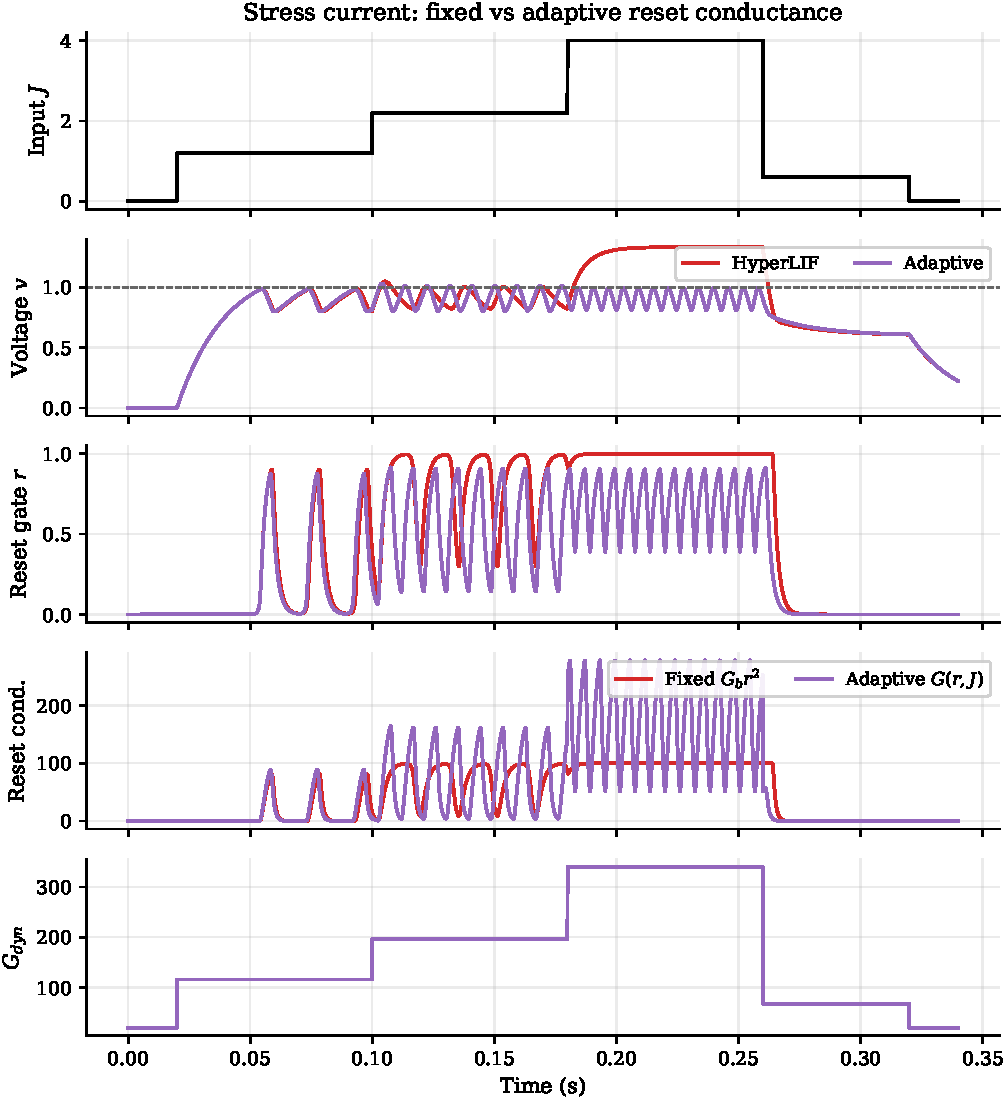
\includegraphics[width=\linewidth]{fig_stress}
  \caption{Stress current. Fixed-gain HyperLIF (red) latches during the
  high-current phase while Adaptive HyperLIF (purple) sustains oscillation; the
  dynamic gain $\Gdyn=\Gbase+\beta|J|$ follows the input staircase. Source:
  \code{02\_hyperlif\_vs\_adaptive.csv}.}
  \label{fig:stress}
\end{figure}

\subsection{Frequency--current response and the depolarization block}
\label{sec:results-fi}
\Cref{fig:fi} and \Cref{tab:sweep} summarize the steady-state response to
constant current. Three regimes are evident. LIF firing increases monotonically
and without bound (runaway). Fixed-gain HyperLIF fires only over a narrow band
($J\in[1.5,2.2]$) and then collapses to zero at $J\approx 2.3$--$2.4$, close to
the open-gate branch estimate $\Jdb=2.4$ from \cref{eq:jdb}; beyond it the mean membrane
voltage climbs linearly as $v^\ast=J/(1+\tau\Gb)=J/3$ (e.g.\ $1.000$ at $J=3$,
$1.333$ at $J=4$), and the gate saturates---the high-voltage latch of
\cref{eq:vstar}. The fixed-point prediction matches the simulated latched voltage
to all reported digits ($1.3333$ vs.\ $1.3333$ at $J=4$). Adaptive HyperLIF fires
over a substantially wider band ($J\in[1.6,3.5]$) with a higher peak rate
($151$ vs.\ $73\,$Hz) and a \emph{bounded} mean voltage near $0.9$, never
exhibiting the high-voltage latch, consistent with \cref{eq:vinf,eq:beta-crit}
($v^\ast_\infty=0.625<0.8$). Honestly, the adaptive model is not unconditionally
firing: with finite $\beta$ it has its own, higher operating ceiling
($J\gtrsim 3.6$ here) above which the bounded oscillation no longer crosses the
default event surface and detected spiking ceases. Crucially, this failure is
bounded---the membrane oscillates below threshold near $0.9$ rather than
latching at $J/3$---so the event channel becomes silent while the continuous
state remains dynamically active.

\begin{figure}[t]
  \centering
  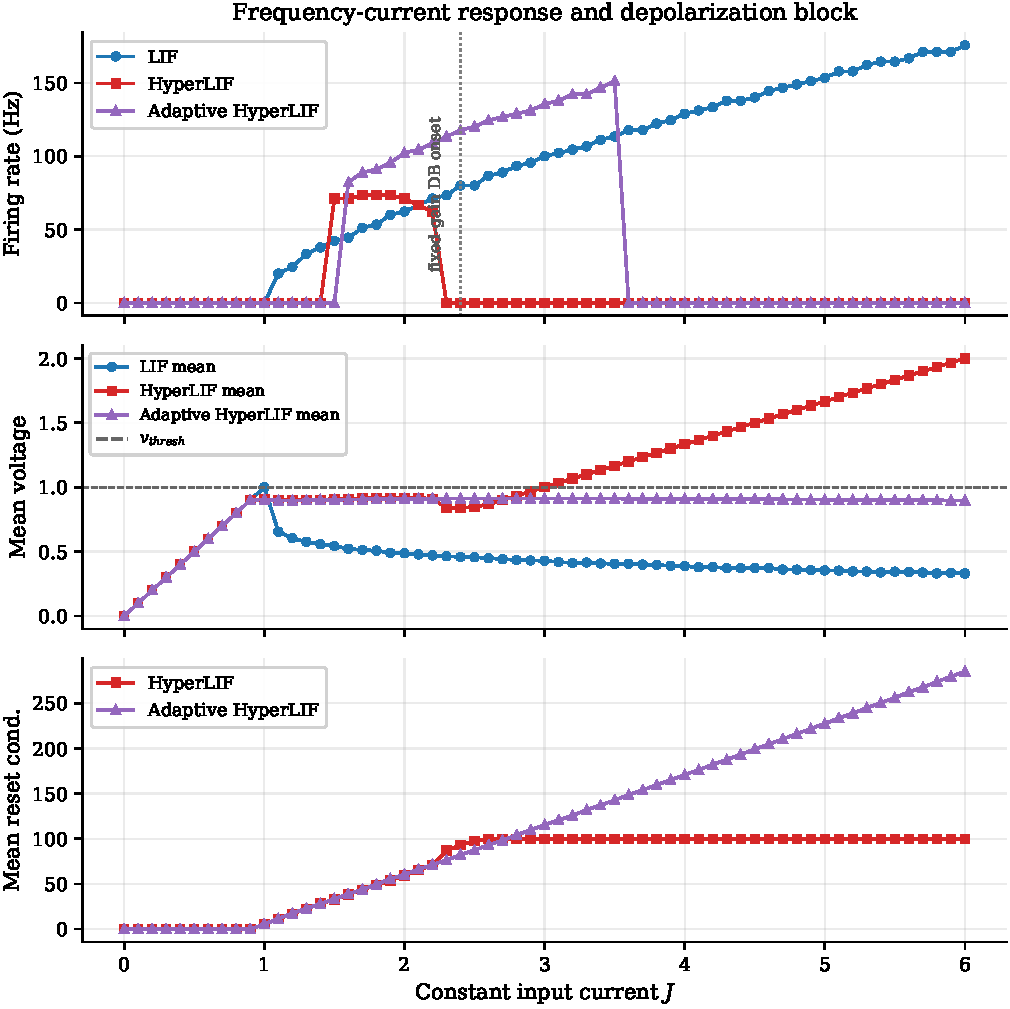
\includegraphics[width=\linewidth]{fig_fi}
  \caption{Frequency--current response. (Top) firing rate: LIF runs away,
  fixed-gain HyperLIF collapses near the open-gate branch estimate $\Jdb=2.4$, Adaptive
  HyperLIF sustains a wider band. (Middle) mean voltage: the HyperLIF latch
  climbs as $J/3$ while Adaptive stays bounded near $0.9$. (Bottom) mean reset
  conductance saturates for HyperLIF but grows with $J$ for Adaptive. Source:
  \code{03\_current\_sweep.csv}.}
  \label{fig:fi}
\end{figure}
\begin{table*}[t]
\centering
\caption{Steady-state response at representative constant currents (from \texttt{03\_current\_sweep.csv}). The fixed-gain HyperLIF firing rate collapses to zero and its mean voltage latches above threshold once $J$ exceeds the analytical depolarization-block onset $J_{\mathrm{DB}}=2.4$, whereas Adaptive HyperLIF sustains spiking with a bounded mean voltage.}
\label{tab:sweep}
\begin{tabular}{cccccc}
\toprule
& \multicolumn{3}{c}{Firing rate (Hz)} & \multicolumn{2}{c}{Mean voltage} \\
\cmidrule(lr){2-4}\cmidrule(lr){5-6}
$J$ & LIF & HyperLIF & Adaptive & HyperLIF & Adaptive \\
\midrule
1 & 0.0 & 0.0 & 0.0 & 0.906 & 0.906 \\
1.5 & 42.2 & 71.1 & 0.0 & 0.908 & 0.903 \\
2 & 62.2 & 71.1 & 102.2 & 0.917 & 0.910 \\
2.4 & 80.0 & 0.0 & 117.8 & 0.840 & 0.912 \\
3 & 100.0 & 0.0 & 135.6 & 1.000 & 0.913 \\
4 & 128.9 & 0.0 & 0.0 & 1.333 & 0.910 \\
\bottomrule
\end{tabular}
\end{table*}


\Cref{fig:db} isolates the contrast at a single sustained drive $J=3.3$ (above
$\Jdb$): the fixed-gain neuron settles to the predicted latched voltage $1.1$
with a saturated gate and emits no further events, while the adaptive neuron
produces a clean limit cycle with $42$ events over $0.3\,$s.

\begin{figure}[t]
  \centering
  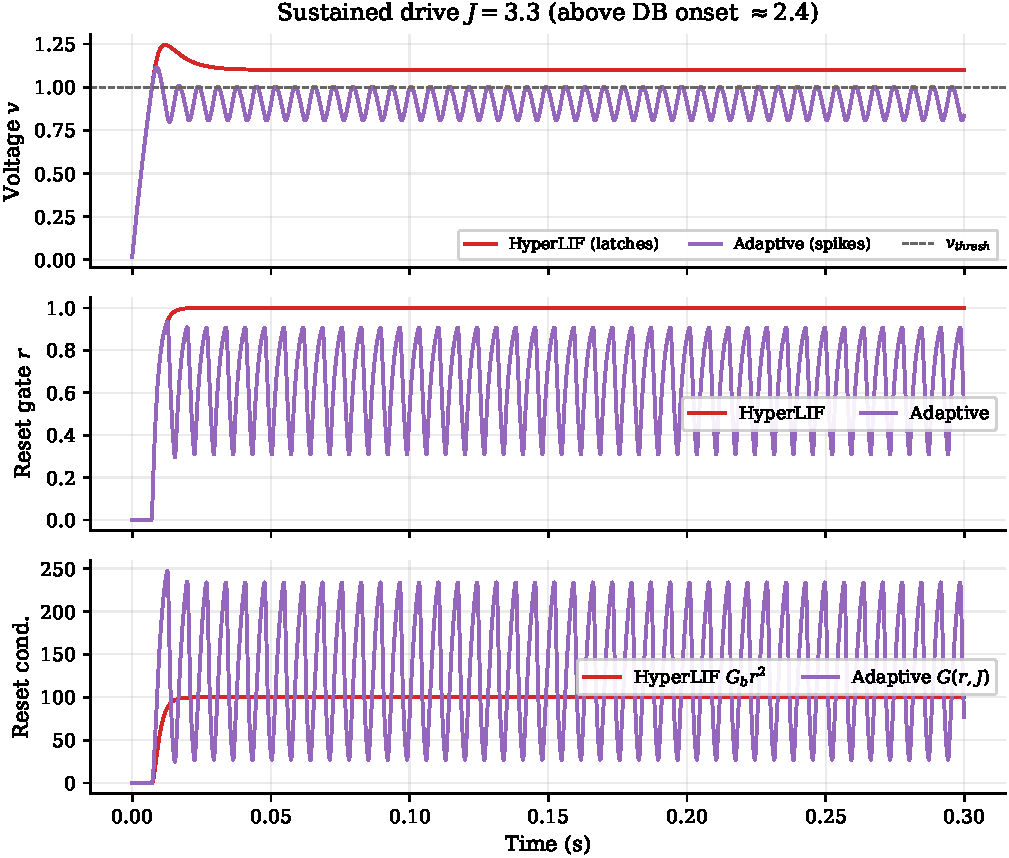
\includegraphics[width=\linewidth]{fig_db}
  \caption{Depolarization-block latch at sustained drive $J=3.3$. Fixed-gain
  HyperLIF (red) latches at $v\approx 1.1$ with a saturated gate; Adaptive
  HyperLIF (purple) maintains a limit cycle. Source:
  \code{04\_depolarization\_block.csv}.}
  \label{fig:db}
\end{figure}

\subsection{Numerical accuracy and stability}\label{sec:results-integration}
\Cref{fig:integration} and \Cref{tab:integration} report the membrane error of
both stepping schemes against the RK4 reference. Both converge at first order in
$\Delta t$, and the gate error is identical because the gate update
\cref{eq:gate-update} is shared. In the convergent regime the explicit and
exponential schemes have comparable accuracy (here the explicit scheme has a
slightly lower trajectory RMSE), so the value of the exponential scheme is not
accuracy but \emph{stability}: \Cref{fig:integration}(b) drives the gate fully
open ($J=4$, $\lambda\approx 150$) and increases $\Delta t$; once
$\lambda\Delta t>2$ the explicit scheme develops growing spurious overshoot
(its maximum $|v|$ rises to $2,3,4,6$ as $\lambda\Delta t$ grows), whereas the
exponential scheme remains bounded near the true latched value $v^\ast=J/3$. This
is why the Nengo port, which must remain well-behaved at arbitrary $\Delta t$ and
high conductance, uses the exponential update.

\begin{figure}[t]
  \centering
  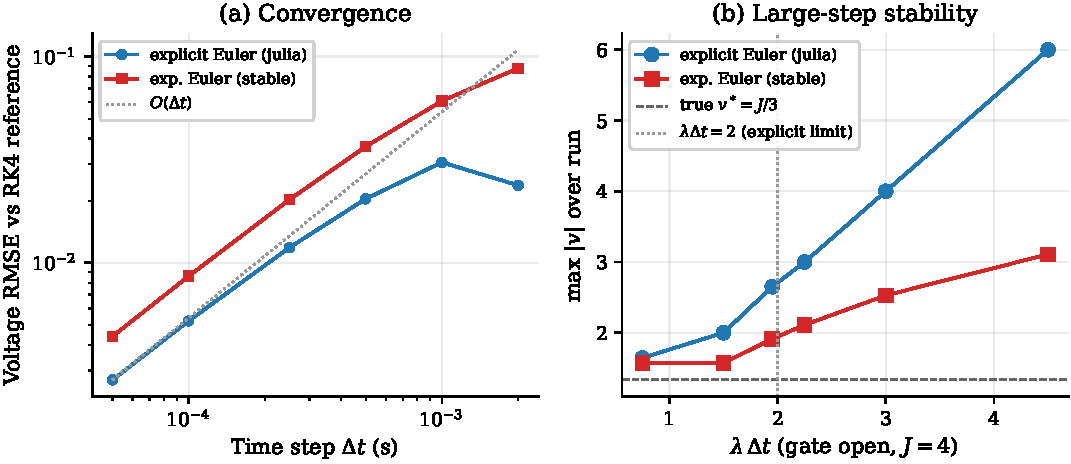
\includegraphics[width=\linewidth]{fig_integration}
  \caption{(a) First-order convergence of both schemes against an RK4 reference
  of the continuous ODE. (b) Large-step stability at $J=4$: explicit Euler
  overshoots once $\lambda\Delta t>2$; the exponential update stays bounded near
  $v^\ast=J/3$. Source: \code{06\_integration\_accuracy.csv},
  \code{06\_stability.csv}.}
  \label{fig:integration}
\end{figure}
\begin{table}[t]
\centering
\caption{Voltage error of the two stepping schemes against a fine RK4 reference of the continuous ODE (from \texttt{06\_integration\_accuracy.csv}). Both converge at first order; the gate update is shared and identical.}
\label{tab:integration}
\begin{tabular}{cccc}
\toprule
$\Delta t$ (s) & RMSE explicit & RMSE exponential & Gate RMSE \\
\midrule
0.002 & 0.0237 & 0.0877 & 0.16 \\
0.001 & 0.0307 & 0.0609 & 0.2 \\
$5.000\!\times\!10^{-4}$ & 0.0204 & 0.0366 & 0.134 \\
$2.500\!\times\!10^{-4}$ & 0.0118 & 0.0202 & 0.0806 \\
$1.000\!\times\!10^{-4}$ & 0.00522 & 0.0086 & 0.0367 \\
$5.000\!\times\!10^{-5}$ & 0.0027 & 0.00439 & 0.0191 \\
\bottomrule
\end{tabular}
\end{table}


\subsection{Python--Nengo parity}\label{sec:results-parity}
\Cref{fig:parity} and \Cref{tab:parity} report the central validation result.
The standalone exponential stepping and the Nengo custom-neuron stepping produce
identical voltage and gate traces, and identical event timing, for both models
and both protocols: the voltage and gate RMSE are exactly $0$, the maximum
absolute voltage/gate difference is exactly $0$, and the event-mismatch count is
$0$. The difference trace in \Cref{fig:parity} is flat at the $10^{-15}$ scale.
Because both implementations call the same numerical kernel
(\Cref{sec:nengo}), this is an algorithmic identity, not a statistical fit---the
strongest form of evidence that the Nengo port \emph{is} the implemented model
rather than an approximation of it.

\begin{figure}[t]
  \centering
  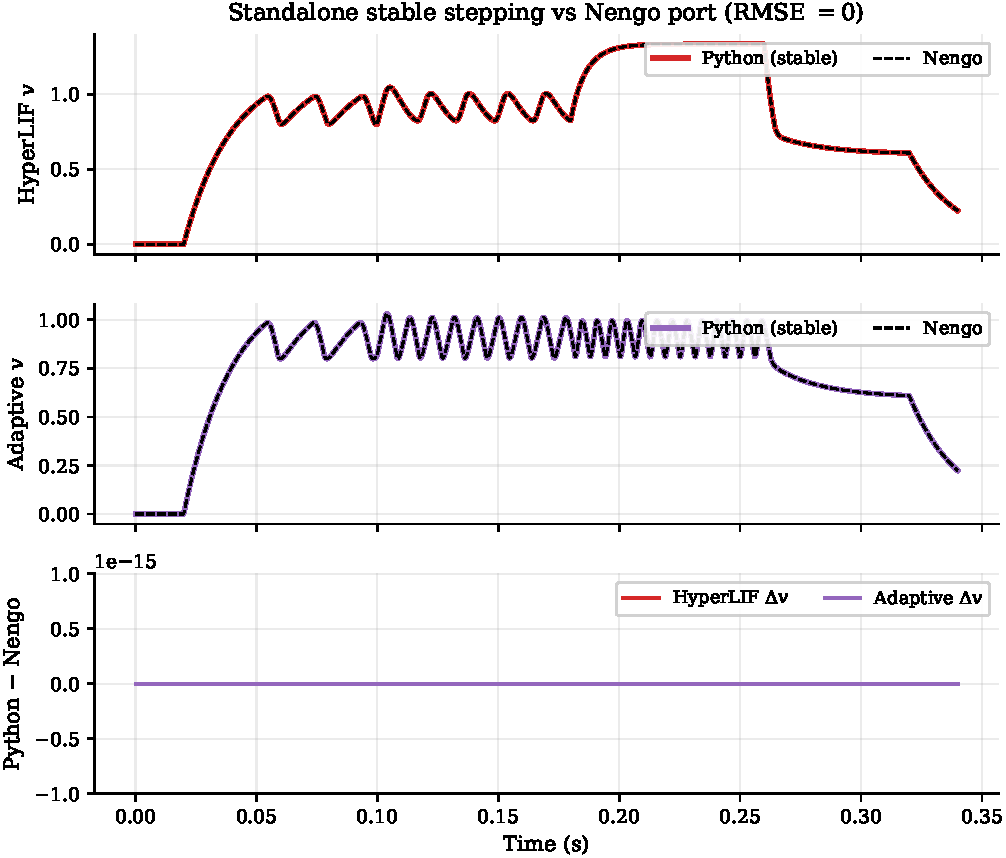
\includegraphics[width=\linewidth]{fig_parity}
  \caption{Standalone stable stepping (thick colored) vs.\ the Nengo port
  (dashed black) for HyperLIF and Adaptive HyperLIF voltage, with the difference
  trace (bottom) flat at machine precision. Source:
  \code{07\_python\_vs\_nengo.csv}, \code{07\_parity\_metrics.csv}.}
  \label{fig:parity}
\end{figure}
\begin{table}[t]
\centering
\caption{Standalone stable stepping vs.\ the Nengo \texttt{NeuronType} port (from \texttt{07\_parity\_metrics.csv}). Agreement is exact to floating point: zero RMSE, zero maximum voltage/gate difference, and zero event-timing mismatches across both protocols and both models.}
\label{tab:parity}
\begin{tabular}{llcccc}
\toprule
Model & Protocol & $v$ RMSE & $\max|\Delta v|$ & $r$ RMSE & Event mism. \\
\midrule
HyperLIF & stress & $0$ & $0$ & $0$ & 0 \\
Adaptive & stress & $0$ & $0$ & $0$ & 0 \\
HyperLIF & step & $0$ & $0$ & $0$ & 0 \\
Adaptive & step & $0$ & $0$ & $0$ & 0 \\
\bottomrule
\end{tabular}
\end{table}


\subsection{Gate-state decoding}\label{sec:results-decode}
\Cref{fig:decode} and \Cref{tab:decoding} compare scalar linear decoders fit to
three internal signals of an Adaptive HyperLIF neuron driven by a smooth current.
A voltage decoder recovers the input current with test RMSE $0.258$; a decoder of
exponentially filtered events does worse ($0.321$), reflecting the sparsity of
the event channel; and a decoder of the reset gate recovers a readiness target
with test RMSE $0.287$. The gate decoder is comparable to the voltage decoder
even though the raw gate is a fast, spiky signal, indicating that the gate
carries genuine, decodable information about proximity to the reset transition.

\begin{figure}[t]
  \centering
  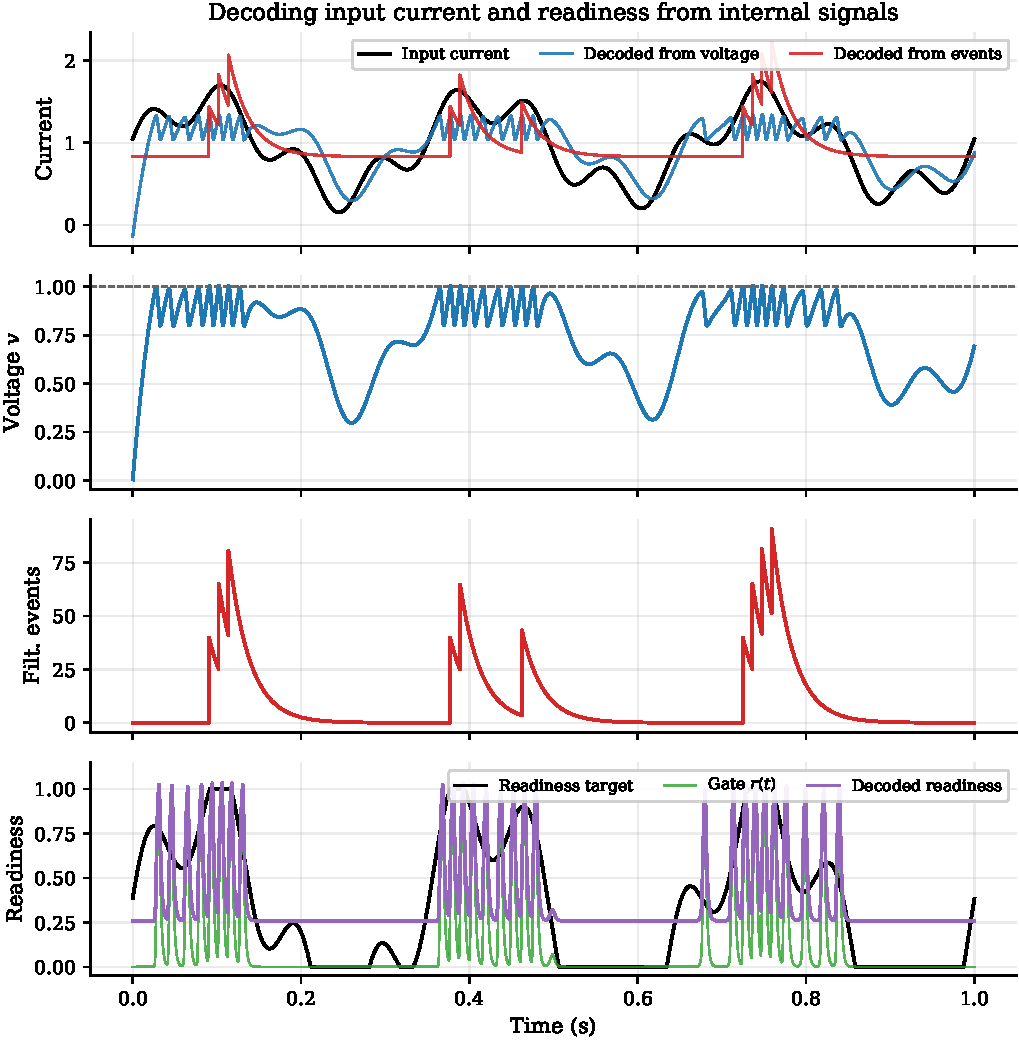
\includegraphics[width=\linewidth]{fig_decode}
  \caption{Decoding from internal signals. (Top) input current and its linear
  decodes from voltage and from filtered events. (Middle panels) the voltage and
  filtered-event features. (Bottom) the readiness target, the raw gate $r(t)$,
  and the gate-based readiness decode. Source:
  \code{05\_gate\_state\_decoding.csv}, \code{05\_decoding\_metrics.csv}.}
  \label{fig:decode}
\end{figure}
\begin{table}[t]
\centering
\caption{Scalar linear decoders fit by least squares with a 70/30 train/test split (from \texttt{05\_decoding\_metrics.csv}).}
\label{tab:decoding}
\begin{tabular}{lcc}
\toprule
Decoder & Train RMSE & Test RMSE \\
\midrule
Voltage $\rightarrow$ input current & 0.293 & 0.258 \\
Filtered events $\rightarrow$ input current & 0.347 & 0.321 \\
Reset gate $\rightarrow$ readiness & 0.283 & 0.287 \\
\bottomrule
\end{tabular}
\end{table}


\subsection{Phase-A NEF app smoke: integrator and oscillator}
\label{sec:results-nef}
The previous sections validate the neuron as a stateful dynamical component.
Paper 3 also asks whether the component can be used inside canonical NEF
networks. As a first smoke test, we replaced the neuron type in two standard
Nengo dynamical models: a one-dimensional recurrent integrator driven by a
short pulse, and a two-dimensional oscillator driven by a brief kick. The test
is deliberately small; it is not an optimized NEF benchmark, but a build/run
check that exercises recurrent decoded dynamics with the custom neuron state.

\begin{table}[t]
  \centering
  \caption{Phase-A NEF application smoke. The integrator value is the mean
  decoded value retained at the end of the pulse experiment; the oscillator
  value is a post-settle standard-deviation amplitude proxy. ``WEAK'' means the
  model built and ran but failed the simple integrator-hold threshold used in
  the smoke script. Source: \code{08\_nef\_app\_smoke.csv}.}
  \label{tab:nef-smoke}
  \begin{tabular}{lccc}
    \toprule
    Neuron & Integrator held & Oscillator std. & Status \\
    \midrule
    LIF & 0.287 & 0.598 & ok \\
    HyperLIF & 0.034 & 0.561 & WEAK \\
    Adaptive HyperLIF & 0.334 & 0.247 & ok \\
    \bottomrule
  \end{tabular}
\end{table}

\Cref{tab:nef-smoke} gives a useful, honest first result. All three neuron
types build and run in both recurrent NEF models, and all three show a
non-trivial oscillator response. LIF and Adaptive HyperLIF also integrate and
hold the pulse. Base HyperLIF, however, holds only \(0.034\), far below the
LIF/Adaptive values, even though it oscillates. This is not a parity failure:
the custom neuron is still exactly the implemented model. It is a readout
availability problem. At the reference event level \(v_{\mathrm{event}}=\vth\),
the base HyperLIF port can emit too few useful events for an NEF recurrent rate
loop. This finding links directly to \Cref{sec:thetaevent}: the continuous
reset dynamics should remain fixed, but the readout event threshold can be
adapted for Nengo communication channels.

We also ran a broader Core-Nengo capability survey using small communication,
function-representation, transform, working-memory, oscillator, and PES-learning
models. To keep this survey executable across many app/variant combinations, the
experiment uses local subclasses with approximate build-time rate curves for
decoder solving; the runtime neuron state equations are unchanged. Thus
\Cref{tab:capability-sweep} is a compatibility and calibration-direction result,
not a final NEF benchmark. All \(54\) app/variant combinations built and ran,
including static-origin variants with \(\vre=-0.6\) and \(\vmin=-2.0\).
For HyperLIF, lowering \(\thetaevent\) from \(1.00\) to \(0.95\) increased event
availability in every app in the sweep (for example, communication-channel
activity rose from \(20.1\) to \(25.9\) Hz/neuron), but did not uniformly improve
decoded accuracy. The static-origin condition was also mixed: at
\(\thetaevent=0.95\), it improved simple communication-channel RMSE for
HyperLIF (\(0.346\to 0.217\)) and improved PES late-error RMSE for both
HyperLIF (\(0.631\to 0.549\)) and Adaptive HyperLIF (\(0.546\to 0.497\)), but
worsened the transform, working-memory, and oscillator smoke metrics. Moreover,
in this fast sweep origin often increased event activity rather than serving as
a clean sparsity dial, indicating that the approximate build-time rate proxy is
not yet origin-aware. This reinforces the central practical lesson:
\(\thetaevent\) is necessary for event availability, while ensemble calibration
and origin-aware rate fitting remain the next optimization problems.
\Cref{sec:capability} carries this calibration through with a fitted operating
point (candidate \code{T023}) and exact settled-rate ensemble builds: the
apparent weaknesses of \Cref{tab:nef-smoke,tab:capability-sweep} are then
resolved, and HyperLIF becomes competitive with---and on dynamics and memory
better than---LIF across the full capability suite. \Cref{tab:nef-smoke,tab:capability-sweep}
should therefore be read as the \emph{un-calibrated} baseline that motivates the
calibrated study, not as the neuron's achievable behavior.

\begin{table}[t]
  \centering
  \caption{Preliminary Core-Nengo capability sweep, using approximate build-time
  rates, \(\thetaevent=0.95\), and static origin
  (\(\vre=-0.6,\vmin=-2.0\)) where marked. Lower is better for RMSE and
  hold-error rows; oscillator standard deviation is an amplitude proxy, not an
  error. Source: \code{10\_core\_nengo\_capability\_sweep.csv}.}
  \label{tab:capability-sweep}
  \small
  \begin{tabular}{llccccc}
    \toprule
    App & Metric & LIF & H 0.95 & H 0.95+orig. & A 0.95 & A 0.95+orig. \\
    \midrule
    Communication & decoded RMSE & 0.156 & 0.346 & 0.217 & 0.235 & 0.326 \\
    Function \(x^2\) & function RMSE & 0.087 & 0.207 & 0.284 & 0.270 & 0.340 \\
    2D transform & transform RMSE & 0.127 & 0.273 & 0.468 & 0.485 & 0.647 \\
    Working memory & hold error & 0.023 & 0.428 & 0.684 & 0.812 & 1.227 \\
    Oscillator & std. amplitude & 0.498 & 0.574 & 0.820 & 0.982 & 1.325 \\
    PES learning & late error RMSE & 0.637 & 0.631 & 0.549 & 0.546 & 0.497 \\
    \bottomrule
  \end{tabular}
\end{table}

% ===========================================================================
\section{Readout Adaptation: Separating theta\_event from the Gate Threshold}
\label{sec:thetaevent}
% ===========================================================================
The NEF smoke test exposes a practical distinction that is easy to miss if one
uses a single threshold for both dynamics and readout. In the implemented model,
\(\vth\) appears inside the gate detector
\(\sigma(\alpha(v-(\vth-\gamma r)))\) and therefore controls the continuous
reset dynamics. The emitted event, by contrast, is a readout signal used by
Nengo decoders and recurrent communication channels. The adaptive-threshold
project therefore introduces a separate event threshold
\(\thetaevent\) while leaving \(\vth\), \(r(t)\), and \(G(r,J)\) unchanged.
This is a readout adaptation, not a new neuron dynamics claim.

\begin{table}[t]
  \centering
  \caption{Static event-threshold sweep from the adaptive-threshold project.
  Moderately lowering the event readout threshold widens the useful settled
  active current band and increases peak settled event rate; lowering it too far
  damages event production. Source:
  \code{09\_theta\_static\_event\_threshold\_summary.csv}, copied from the
  adaptive-threshold project, and \code{docs/PHASE\_RESULTS.md}.}
  \label{tab:theta-static}
  \begin{tabular}{ccc}
    \toprule
    \(\thetaevent\) & Active current band & Peak settled rate \\
    \midrule
    1.00 & 1.60--3.50 & 151.14 Hz \\
    0.98 & 1.20--4.90 & 186.71 Hz \\
    0.95 & 1.00--6.00 & 217.83 Hz \\
    0.90 & 1.00--6.00 & 217.83 Hz \\
    0.80 & 1.10--1.50 & 75.57 Hz \\
    \bottomrule
  \end{tabular}
\end{table}

\Cref{tab:theta-static} shows the main readout result. The baseline event level
\(\thetaevent=1.00\) produces a peak settled rate of \(151.14\) Hz over the
active band \(J\in[1.60,3.50]\). Setting \(\thetaevent=0.95\) widens the active
band to \(J\in[1.00,6.00]\) and raises the peak settled rate to \(217.83\) Hz.
This directly addresses the sparse-event issue observed in
\Cref{sec:results-nef}. The falsification result is equally important:
\(\thetaevent=0.80\), near the gate knee, reduces the active band and lowers the
peak settled rate to \(75.57\) Hz. The paper therefore should not claim that
``lower is better.'' The useful statement is narrower and better: a moderately
lowered readout threshold can increase useful Nengo event availability without
changing the validated continuous reset.

The same project also tested whether event count alone predicts decoder
quality. It does not. Static \(\thetaevent=0.95\) improves the event-only
current decoder relative to \(\thetaevent=1.00\) (test RMSE \(0.2663\) vs.
\(0.3210\)), but a first untuned adaptive threshold produced many more events
with worse event-only decoding. A tuned adaptive rule recovered the research
value: with \(\theta_{\mathrm{base}}=0.99\), target rate \(60\) Hz, error gain
\(0.002\), and spike increment \(0.0005\), the event-only decoder reached test
RMSE \(0.2343\) and the combined state decoder reached \(0.1805\), both better
than the static \(0.95\) baseline in that single-neuron protocol.
\Cref{tab:nef-decoder-ablation} below supplies the first multi-neuron,
seed-matched NEF validation for the calibrated static-\(\thetaevent\) candidates;
the tuned adaptive-threshold rule remains exploratory until repeated at the same
ensemble scale.

% ===========================================================================
\section{HyperLIF Across Nengo: Calibration, Capability Coverage, and Portability}
\label{sec:capability}
% ===========================================================================
We now ask directly whether HyperLIF is usable across the breadth of Nengo, and
where the limits lie---both of the neuron and of the framework. Two changes
sharpen the picture from the Phase-A smoke of \Cref{sec:results-nef}: proper
ensemble calibration, and testing every capability class against every
simulation backend. The capability, backend, PES, and seed-preflight evidence is
traceable to the project CSV/log artifacts and is summarized in the
reproducibility map rather than embedded as long file paths in the text.

\subsection{Operating-point calibration removes the apparent weakness}
The Phase-A smoke (\Cref{tab:nef-smoke}) reported base HyperLIF as a weak
integrator (\(0.034\)). We now show this was an \emph{operating-point} artifact,
not a dynamics limitation. Using a readout-calibrated ensemble build
(\(\thetaevent=0.95\), static origin \(\vre=-0.6\), and a fitted rate-to-current
gain of \(140\)---candidate \code{T023} from an origin-aware calibration sweep of
\(126\) app--candidate runs), HyperLIF integrates and holds (\(0.003\)), and on an
amplitude-matched oscillator and a gated working memory it matches or
\emph{exceeds} LIF (\Cref{tab:capability-calib}). Among the HyperLIF family,
\code{T023} is the strongest general-purpose candidate: over the six-app
calibration suite it is the only non-LIF configuration with zero bad-app columns,
and its robustness score (\(1.25\)) is closest to native LIF (\(0.68\)). The
continuous reset dynamics are unchanged and parity remains exact; only the
ensemble operating point moved. This is the central practical lesson: for a
continuous-reset neuron, usable NEF behavior is a calibration problem
(\(\thetaevent\), origin, gain), not a change to the core equations.

\begin{table}[t]
  \centering
  \caption{Calibrated capability coverage: every canonical Nengo capability runs
  with HyperLIF as a drop-in \code{NeuronType}. Values are task error (lower is
  better; oscillator and amplitude rows are amplitude-error proxies). HyperLIF
  and Adaptive use the calibrated \code{T023}/\code{T033} operating point. Once
  calibrated, HyperLIF \emph{beats} LIF on the oscillator and working memory, and
  is exact on action selection; the one weakness is PES online learning
  (\Cref{sec:capability-trade}). Across representation apps HyperLIF fires
  \(\approx 33\) Hz vs LIF's \(\approx 120\) Hz (\(\sim\!3.5\times\) sparser).
  Source: \code{13\_hyperlif\_nengo\_capability\_matrix.csv}.}
  \label{tab:capability-calib}
  \small
  \begin{tabular}{llccc}
    \toprule
    Capability & App (metric) & LIF & HyperLIF & Adaptive \\
    \midrule
    NEF repr. & comm.\ (RMSE)        & 0.193 & 0.211 & 0.205 \\
    NEF repr. & function (RMSE)      & 0.194 & 0.222 & 0.200 \\
    NEF repr. & transform (RMSE)     & 0.197 & 0.211 & 0.209 \\
    NEF dyn.  & integrator (hold)    & 0.001 & 0.003 & 0.010 \\
    NEF dyn.  & oscillator (amp.)    & 0.147 & \textbf{0.100} & 0.164 \\
    Memory    & gated (hold)         & 0.033 & \textbf{0.019} & 0.035 \\
    Learning  & PES (late RMSE)      & \textbf{0.051} & 0.445 & 0.102 \\
    Cognition & binding (\(1-\cos\)) & 0.014 & 0.054 & 0.011 \\
    Cognition & action sel.\ (err)   & 0.000 & 0.000 & 0.000 \\
    \bottomrule
  \end{tabular}
\end{table}

\Cref{tab:capability-seeded} adds a seed-matched preflight layer to the
calibrated matrix. The run repeats seven core applications for native LIF,
uncalibrated HyperLIF, calibrated HyperLIF \code{T023}, and calibrated Adaptive
HyperLIF \code{T033}; all 84 simulations completed without failure. The
result confirms the calibration thesis without overclaiming a leaderboard:
\code{T023} is the best low-rate HyperLIF candidate for representation and
dynamics, \code{T033} is the better HyperLIF-family candidate for working memory
and PES learning, and the uncalibrated \(\thetaevent=1.00\) HyperLIF row remains
useful mainly as a cautionary sparsity baseline.

\begin{table*}[t]
  \centering
  \caption{Three-seed core capability preflight. Each cell reports task error
  mean \(\pm\) standard deviation with mean firing rate in Hz in parentheses.
  All rows have \(n=3\) seeds and zero failures. Source:
  \code{17\_capability\_seed\_sweep\_summary.csv}.}
  \label{tab:capability-seeded}
  \scriptsize
  \begin{tabular}{llccc}
    \toprule
    App & Metric & LIF & HyperLIF \code{T023} & Adaptive \code{T033} \\
    \midrule
    Integrator & hold error & \(0.0118\pm0.0039\) (87.4) & \(\mathbf{0.0037\pm0.0039}\) (39.1) & \(0.0089\pm0.0060\) (46.6) \\
    Oscillator & amplitude error & \(0.1543\pm0.0042\) (114.8) & \(\mathbf{0.0672\pm0.0310}\) (38.3) & \(0.1656\pm0.0066\) (60.8) \\
    Communication & decode RMSE & \(\mathbf{0.1934\pm0.0003}\) (120.3) & \(0.2030\pm0.0013\) (33.6) & \(0.2037\pm0.0012\) (63.2) \\
    Function & function RMSE & \(\mathbf{0.1937\pm0.0002}\) (118.5) & \(0.2299\pm0.0069\) (32.2) & \(0.2004\pm0.0006\) (61.8) \\
    Transform & transform RMSE & \(\mathbf{0.1963\pm0.0010}\) (118.2) & \(0.2079\pm0.0038\) (33.1) & \(0.2087\pm0.0005\) (62.0) \\
    Working memory & hold error & \(0.0292\pm0.0039\) (103.5) & \(0.0368\pm0.0169\) (40.7) & \(\mathbf{0.0291\pm0.0086}\) (54.9) \\
    PES learning & late RMSE & \(\mathbf{0.0489\pm0.0020}\) (117.9) & \(0.4393\pm0.0119\) (33.9) & \(0.1025\pm0.0031\) (62.9) \\
    \bottomrule
  \end{tabular}
\end{table*}

\subsection{State-readout decoder ablation}
\label{sec:capability-decoders}
\Cref{tab:nef-decoder-ablation} asks a narrower but important question than the
capability tables: once the calibrated HyperLIF neurons are inside a Nengo
ensemble, which observable state channels are useful for decoding a represented
scalar signal? We repeat a one-dimensional NEF communication channel over five
network seeds and fit offline ridge decoders from filtered spikes, membrane
voltage, reset gate, and combined feature sets. This is not a replacement for
Nengo's solved decoders and not a controller result; it is a state-readout
ablation showing what the probeable HyperLIF variables make available.

\begin{table*}[t]
  \centering
  \caption{Five-seed scalar NEF state-readout ablation. Each entry is test RMSE
  mean \(\pm\) sample standard deviation for decoding the represented scalar
  signal from the listed features; lower is better. Column headers report mean
  firing rate. HyperLIF uses calibrated \code{T023}; Adaptive uses calibrated
  \code{T033}. Source:
  \code{18\_nef\_decoder\_state\_ablation\_summary.csv}.}
  \label{tab:nef-decoder-ablation}
  \scriptsize
  \setlength{\tabcolsep}{4pt}
  \begin{tabular}{lccc}
    \toprule
    Feature set & LIF (100.5 Hz) & HyperLIF \code{T023} (40.3 Hz) & Adaptive \code{T033} (53.3 Hz) \\
    \midrule
    Nengo decoded output & \(0.2269\pm0.0004\) & \(0.2273\pm0.0047\) & \(0.2339\pm0.0012\) \\
    Filtered spikes & \(0.3200\pm0.0071\) & \(0.3252\pm0.0096\) & \(0.3228\pm0.0100\) \\
    Voltage & \(0.1830\pm0.0045\) & \(0.2726\pm0.0203\) & \(0.2387\pm0.0085\) \\
    Reset gate & --- & \(0.1110\pm0.0064\) & \(0.1269\pm0.0073\) \\
    Spikes + voltage & \(0.3237\pm0.0242\) & \(0.1735\pm0.0232\) & \(\mathbf{0.0973\pm0.0161}\) \\
    Voltage + gate & --- & \(0.1237\pm0.0288\) & \(0.2089\pm0.0197\) \\
    Spikes + voltage + gate & --- & \(\mathbf{0.1106\pm0.0212}\) & \(0.1167\pm0.0141\) \\
    \bottomrule
  \end{tabular}
\end{table*}

Two points follow. First, the normal Nengo decoded outputs are essentially tied
for LIF, calibrated HyperLIF, and calibrated Adaptive HyperLIF, while HyperLIF
uses about \(2.5\times\) fewer spikes than LIF and Adaptive about \(1.9\times\)
fewer. Second, the continuous states are not merely diagnostic: for the
calibrated HyperLIF-family neurons, reset-gate and combined-state readouts decode
the scalar channel substantially better than filtered spikes alone. This supports
using \(r(t)\) as a state feature, while leaving task-specific residual-control
targets to future closed-loop experiments.

\subsection{The efficiency--learning-speed trade}
\label{sec:capability-trade}
The one durable weakness is online-learning speed. In a matched-time PES
channel-learning task, HyperLIF converges more slowly than LIF (late error
\(0.445\) vs \(0.051\); \Cref{fig:capability}a). This is a firing-rate effect and
is itself a tunable operating point: sweeping the readout gain
(\Cref{fig:capability}b) reveals a sweet spot near \(40\) Hz where late error
falls sevenfold (\(0.85\to 0.12\)), but an honest ceiling remains---HyperLIF's
intrinsic sparsity peaks below LIF's rate, so learning stays slower even when
optimally tuned. The same sparsity that buys \(\sim\!3.5\times\) representation
efficiency costs online-learning speed: one trade, seen from both sides. The
higher-rate Adaptive variant recovers much of the gap (\(0.102\)).

\begin{figure}[t]
  \centering
  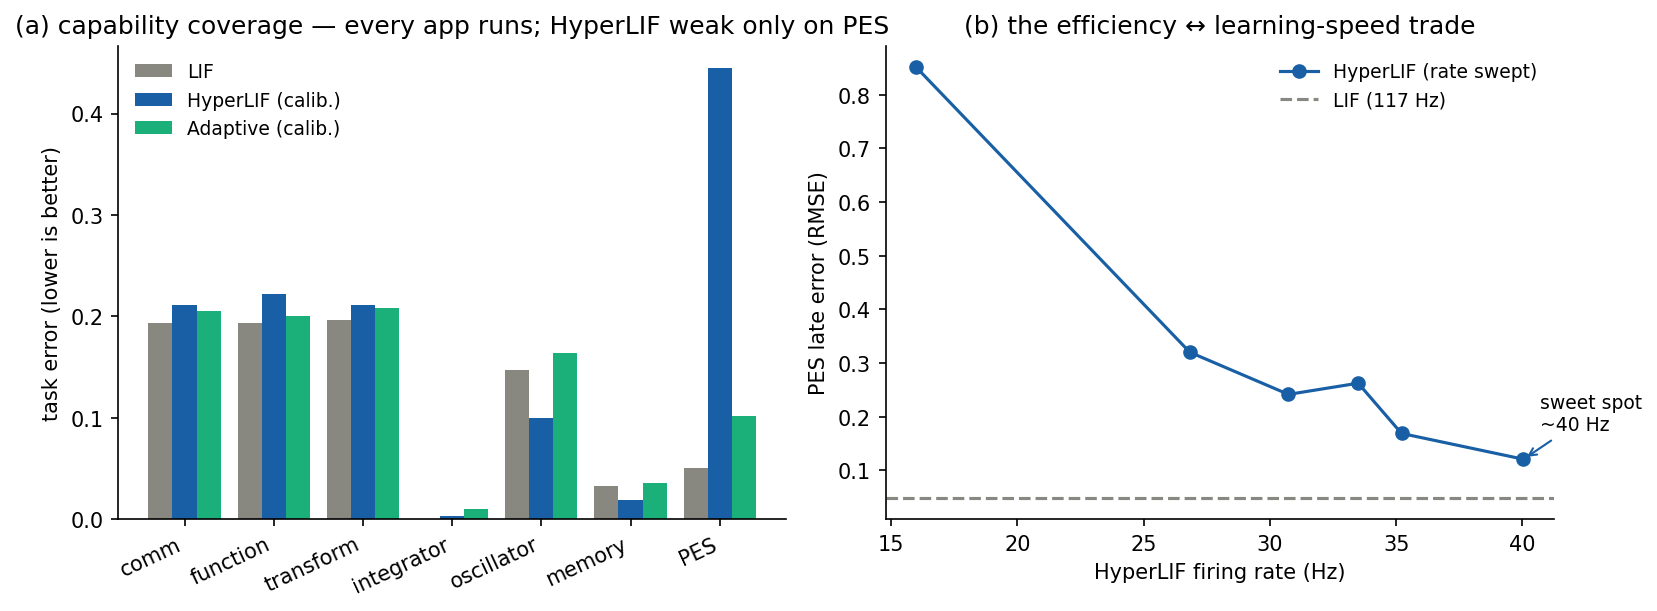
\includegraphics[width=\linewidth]{figures/fig_nengo_capability.png}
  \caption{(a) Task error per Nengo capability, LIF vs calibrated HyperLIF vs
  Adaptive: every app runs; HyperLIF is competitive or better except on PES
  online learning. (b) The efficiency\,\(\leftrightarrow\)\,learning-speed trade:
  sweeping HyperLIF's firing rate gives a sweet spot near \(40\) Hz, but its
  sparsity ceiling keeps it above the LIF reference.}
  \label{fig:capability}
\end{figure}

\subsection{Backend portability: the framework limit}
\label{sec:capability-backend}
A custom continuous-gate \code{NeuronType} is not portable across Nengo's
accelerated and hardware backends (\Cref{tab:backend}). On a machine with a
working OpenCL device---native LIF runs on the GPU---NengoOCL rejects HyperLIF
(\emph{``unsupported neuron type''}) because no OpenCL kernel exists for it;
NengoLoihi rejects it at build validation (\emph{``cannot be simulated on
Loihi''}) because a continuous two-state gate is not in the fixed hardware neuron
set, and the same wall applies to FPGA targets; and NengoDL---the one backend
where a custom neuron is in principle \emph{trainable} via a TensorFlow builder
---could not be exercised on a current software stack, as \code{nengo-dl} is
version-locked to Keras~2 and \code{protobuf}~3. HyperLIF is therefore a
first-class citizen of the reference NumPy simulator, where every capability
above runs, but is confined to it: accelerated execution would require a
hand-written per-backend kernel, and neuromorphic deployment is precluded by the
fixed hardware neuron model. This is a limitation of continuous-dynamics custom
neurons in the Nengo ecosystem generally, not specific to HyperLIF.

\begin{table}[t]
  \centering
  \caption{Backend portability probe: the same minimal ensemble, LIF vs
  HyperLIF, on each backend. Source: \code{14\_backend\_portability\_probe.py}.}
  \label{tab:backend}
  \small
  \begin{tabular}{lll}
    \toprule
    Backend & LIF & HyperLIF \\
    \midrule
    NengoCore (NumPy)   & runs & \textbf{runs} \\
    NengoOCL (GPU)      & runs & rejected: no kernel \\
    NengoLoihi / FPGA   & ---  & rejected: fixed neuron set \\
    NengoDL (TensorFlow)& ---  & blocked: version-lock \\
    \bottomrule
  \end{tabular}
\end{table}

% ===========================================================================
\section{Interpretation: Gate-State Readiness-to-Fire}\label{sec:readiness}
% ===========================================================================
The reset gate is more than an internal bookkeeping variable. By
\cref{eq:theta,eq:sigmoid}, $r$ tracks $\sigma(\alpha(v-(\vth-\gamma r)))$: it
rises as the membrane approaches the (hysteresis-lowered) threshold and saturates
once the reset trajectory is committed. It is therefore a continuous
\emph{readiness-to-fire} signal: small $r$ means far from the reset transition,
rising $r$ means approaching it, and saturated $r$ means the reset is fully
engaged. Two observations from \Cref{sec:results} make this concrete. First, in
\Cref{fig:step} the gate completes several readiness cycles while the event
channel reports a single spike---the gate exposes sub-threshold structure that
spikes discard. Second, \Cref{tab:decoding} shows that a linear gate decoder is
competitive with a voltage decoder for a readiness target, and
\Cref{tab:nef-decoder-ablation} extends the point to a scalar NEF ensemble:
calibrated HyperLIF-family reset-gate and combined-state readouts decode the
represented signal at low firing rates. Unlike the voltage, whose interpretation
near reset is ambiguous in a hard-reset neuron, the gate is a bounded $[0,1]$
quantity with a direct interpretation in terms of the effective threshold. This
makes $r(t)$ a natural \emph{residual feature} to augment spike/rate features in
downstream estimation.

% ===========================================================================
\section{Connection to Residual Augmentation and Quaternion Attitude Control}
\label{sec:bridge}
% ===========================================================================
We now outline the intended application, and we are explicit that this section
is \emph{forward-looking}: no closed-loop control results are claimed here. The
NEF pipeline that Nengo implements suggests a direct route to using HyperLIF
neurons inside an attitude controller. An attitude error---for example a
quaternion error vector between the estimated and desired
orientations~\cite{markley2014attitude}---is encoded as input current $J$ to a
HyperLIF ensemble; the ensemble's spikes, membrane voltages, and reset gates are
decoded into control or residual features; and a controller maps those features
to torques. NEF-based spiking networks have already been shown to learn adaptive
control signals online~\cite{dewolf2016reach}, and the state-readout ablation of
\Cref{tab:nef-decoder-ablation} shows that the gate is already decodable in a
scalar NEF channel. The intended control extension is:
\begin{equation}
  \text{error} \to J \to (v, r, \text{spikes}) \to \text{decoded residual} \to \text{torque}.
  \label{eq:pipeline}
\end{equation}
The hypothesis to be tested in future work is that a task-specific gate-state
residual term improves tracking or robustness relative to spike-only or
voltage-only decoding, because $r(t)$ encodes readiness information that the
event channel omits (\Cref{sec:readiness}). The validated \code{NeuronType} port and the exact
parity result of \Cref{sec:results-parity} are precisely what make such a study
trustworthy: any controller behavior can be attributed to the model, not to an
implementation discrepancy. The present paper deliberately keeps the neuron
reference free of controller code; the controller stage will import this
reference rather than re-define the equations.

% ===========================================================================
\section{Limitations}\label{sec:limitations}
% ===========================================================================
We list the limitations plainly. (i) Most validation is performed on a single
neuron driven by injected current; the later Nengo capability experiments use
compact ensembles and seed-matched preflights, not paper-scale task optimization,
and closed-loop control is not evaluated here. (ii) The parameters in
\Cref{tab:params} are a
normalized reference set chosen for clean demonstration; they differ from the
benchmark-scale training parameters of~\cite{hyperlif_theory}, so the specific
numbers ($\Jdb=2.4$, $\beta_{\mathrm{crit}}=62.5$, etc.) are parameter-dependent
instances of the general relations \cref{eq:jdb,eq:beta-crit}, not universal
constants. (iii) The DB analysis uses a frozen-gate fixed-point argument; it
correctly predicts the onset and latched voltage observed in simulation but is a
sufficient-condition characterization rather than a full bifurcation analysis,
and the adaptive ceiling above $J\approx 3.6$ is reported empirically. (iv) The
decoder studies use deliberately simple linear/ridge fits: one single-neuron
readiness study and one five-seed scalar NEF channel. They validate state
availability and decodability, not optimized high-dimensional task decoders. (v) The
\(\thetaevent\) results are readout-level results from the adaptive-threshold
project; static \(0.95\) is a practical baseline and the tuned adaptive rule is
still exploratory until validated in ensembles. (vi) The
attitude-control connection of \Cref{sec:bridge} is a design and a hypothesis,
not a result. (vii) The explicit-Euler scheme, included for reference fidelity,
is only conditionally stable (\Cref{sec:results-integration}). (viii) HyperLIF's
usable NEF behavior is operating-point-dependent: the calibrated results of
\Cref{sec:capability} require a fitted rate-to-current gain together with
\(\thetaevent\)/origin settings, and its online-learning (PES) convergence is
slower than LIF's at matched time---a firing-rate trade rather than a fixed
deficit. (ix) The component is confined to the reference NumPy simulator: the
OpenCL, Loihi, and TensorFlow backends do not currently accept a custom
continuous-gate neuron (\Cref{sec:capability-backend}), so accelerated or
neuromorphic deployment is out of scope for this paper.

% ===========================================================================
\section{Future Work}\label{sec:future}
% ===========================================================================
The natural next steps are: (a) extend the current capability suite beyond the
seeded seven-app core and nine-app matrix to controlled Lorenz dynamics,
larger-scale NengoSPA tasks, and control examples; (b) extend the scalar
state-readout ablation of \Cref{tab:nef-decoder-ablation} to higher-dimensional
channels, readiness targets, tuned adaptive thresholds, and residual-control
targets; (c) reserve a five-seed capability run for venues or reviewers that
require broader statistical margins, since the completed three-seed preflight is
already sufficient for the present implementation-and-methods claim; (d)
closed-loop quaternion attitude control following
\cref{eq:pipeline}, with repeated, seed-matched trials and paper-scale
statistics; (e) mapping the gate $r(t)$ to local, multi-factor plasticity rules
as a low-memory alternative to backpropagation through time, as suggested
in~\cite{hyperlif_theory}; and (f) the backend/hardware engineering that
\Cref{sec:capability-backend} shows is currently required for any target beyond
the reference simulator---a hand-written OpenCL kernel for NengoOCL, a
TensorFlow \code{NeuronBuilder} (and a maintained \code{nengo-dl}) for NengoDL,
and, for Loihi/FPGA, a mapping of the continuous gate onto a fixed hardware
neuron model, which is the hardest and possibly infeasible case.

% ===========================================================================
\section{Conclusion}\label{sec:conclusion}
% ===========================================================================
We presented a clean, equation-faithful, and rigorously validated reference
implementation of the HyperLIF and Adaptive HyperLIF continuous-reset neurons,
compatible with Nengo. Every manuscript equation is realized in code; a
frozen-open-gate analysis gives the branch estimate
$\Jdb=(\vth-\gamma)(1+\tau\Gb)$ and branch voltage $J/(1+\tau\Gb)$; the latter
matches the simulated high-drive latch. The adaptive conductance law bounds the
positive-drive, $r=1$ asymptotic branch below the gate knee when
$\beta>1/(\tau(\vth-\gamma))$, changing the high-drive regime without proving
global stability or indefinite firing. The two stepping schemes
are characterized for accuracy and stability, and the Nengo port reproduces the
standalone model to floating-point exactness.

Placing the neurons across the breadth of Nengo, we found that the apparent
weakness of base HyperLIF in canonical models is an operating-point artifact:
with readout calibration (\(\thetaevent\), origin, and a fitted rate-to-current
gain) HyperLIF runs all nine canonical capability classes---representation,
dynamics, memory, online learning, and cognition---matching or exceeding LIF on
dynamics and memory at roughly \(3.5\times\) fewer spikes. A three-seed core
preflight completed 84/84 Nengo simulations with zero failures and confirmed the
main trade: calibrated HyperLIF is the low-rate computation candidate, while the
adaptive variant recovers much of the PES-learning gap. A five-seed scalar NEF
state-readout ablation then showed that the probeable reset gate and combined
state features carry useful represented-signal information at low firing rates.
We also delimited a hard
framework
boundary: a custom continuous-gate neuron runs only in the reference simulator,
as the OpenCL, Loihi, and TensorFlow backends cannot currently accept it.
Interpreting the reset gate as a decodable readiness-to-fire signal, we outlined
a validated-substrate path toward gate-state residual decoding for control, which
we leave as future work. The complete project
regenerates every figure, table, and number from the included code and data.

% ===========================================================================
\appendix
\section{Parameters}\label{app:params}
\Cref{tab:params} lists the default parameters, reflected directly from the
\code{LIFParams}, \code{HyperLIFParams}, and \code{AdaptiveHyperLIFParams}
dataclasses, so the table cannot drift from the implementation.
\begin{table*}[t]
\centering
\caption{Default parameters of the reference implementation, reflected directly from the \texttt{LIFParams}, \texttt{HyperLIFParams}, and \texttt{AdaptiveHyperLIFParams} dataclasses. All voltages and gains are in the normalized convention ($v_{\mathrm{rest}}=v_{\mathrm{reset}}=0$, $v_{\mathrm{thresh}}=1$); $J$ and $G$ are dimensionless relative to the leak.}
\label{tab:params}
\begin{tabular}{llccc}
\toprule
Parameter & Symbol & LIF & HyperLIF & Adaptive HyperLIF \\
\midrule
Membrane time constant & $\tau$ (s) & 0.02 & 0.02 & 0.02 \\
Refractory period & $\tau_{\mathrm{ref}}$ (s) & 0.002 & -- & -- \\
Resting potential & $v_{\mathrm{rest}}$ & 0 & 0 & 0 \\
Reset potential & $v_{\mathrm{reset}}$ & 0 & 0 & 0 \\
Threshold & $v_{\mathrm{thresh}}$ & 1 & 1 & 1 \\
Gate steepness & $\alpha$ & -- & 100 & 100 \\
Gate time constant & $\tau_r$ (s) & -- & 0.002 & 0.002 \\
Hysteresis factor & $\gamma$ & -- & 0.2 & 0.2 \\
Fixed reset gain & $G_b$ & -- & 100 & -- \\
Baseline reset gain & $G_{\mathrm{base}}$ & -- & -- & 20 \\
Adaptive scaling & $\beta$ & -- & -- & 80 \\
Spike amplitude & $A$ & 1 & 1 & 1 \\
Min.\ voltage clamp & $v_{\min}$ & 0 & 0 & 0 \\
\bottomrule
\end{tabular}
\end{table*}


\section{Equation-to-Code Map}\label{app:map}
\begin{sloppypar}
\Cref{eq:lif-ode,eq:lif-update} correspond to \code{src/neurons/lif.py}
(\code{\_lif\_voltage\_update}, \code{simulate\_lif}).
\Cref{eq:theta,eq:sigmoid,eq:gate-ode,eq:hyperlif-ode,eq:gate-update,%
eq:stable-update,eq:euler-update} correspond to \code{src/neurons/hyperlif.py}
(\code{gate\_target}, \code{exact\_gate\_update}, \code{stable\_voltage\_update},
\code{HyperLIFNeuron.step}).
\Cref{eq:adaptive-gain,eq:adaptive-ode} correspond to
\code{src/neurons/adaptive\_hyperlif.py}.
The Nengo realization of \Cref{alg:step} is in
\code{src/neurons/nengo\_hyperlif.py} (\code{HyperLIFNengo.step},
\code{AdaptiveHyperLIFNengo.step}).
\Cref{eq:vstar,eq:jdb,eq:vinf,eq:beta-crit} are implemented and validated in
\code{src/analysis/depolarization\_block.py} and exercised by
\code{experiments/03\_current\_sweep.py}. A line-level table is maintained in
the accompanying \code{MATH\_CODE\_MAP.md}.
\end{sloppypar}

\section{Reproducibility}\label{app:repro}
From the project root, after creating the environment
(\code{scripts/setup\_env.ps1}):
\begin{quote}\small\ttfamily
python experiments/run\_all.py\\
python figures/make\_figures.py\\
python tables/make\_tables.py\\
scripts/build\_paper.ps1
\end{quote}
This regenerates all CSV/logs, all figures (PNG\,+\,PDF), all LaTeX tables, and
compiles this document. See \code{REPRODUCIBILITY.md} and \code{RUNNERS.md} for
details and \code{RESULTS\_AUDIT.md} for the validated/exploratory and
paper-ready/future-work classification of every claim.

% ===========================================================================
\bibliographystyle{IEEEtran}
\bibliography{references}

\end{document}
